\subsection{}
In the long run, firms can change all their inputs.
Capital and labour are not fixed.\\
Technical efficiency occurs when a given number of inputs are combined in such a way as to maximize the level of output.
Technical efficiency is not enough for profits to be maximized. To maximize profit,
the firm chooses among the many technically efficient options. The firm uses the technically efficient option that has the lowest cost.
To maximize profits, the firm chooses the lowest cost combination of labour and capital.\\
They change their inputs in relation to marginal production of capital (MPK) and marginal production of labour (MPL).\\
If MPK $>$ MPL, the firm will increase capital and decrease labour until $\frac{MPK}{P_K} = \frac{MPL}{P_L}$.\\
$\frac{MPK}{P_K} = \frac{MPL}{P_L}$ is called technical efficiency.\\
$\frac{MPK}{MPL} = \frac{P_K}{P_L}$ is called the marginal rate of technical substitution (MRTS).\\
At a given output, minimizing costs maximizes profits.\\
The principle of substitution is the principle that methods of production will change if relative prices of inputs change,
with relatively more of the cheaper input and relatively less of the more expensive input being used.
\par
Long run average cost (LRAC) is connected to the short run average cost (SRAC).\\
Convex hull is the LRAC curve formed from the SRAC curves.\\
Increasing returns to scale (IRS) or economics of scale is when LRAC decreases as output increases (doubling inputs, more than doubles the quantity).\\
Constant returns to scale (CRS) is when LRAC remains constant as output increases (doubling inputs, doubles the quantity).\\
Decreasing returns to scale (DRS) or diseconomies of scale is when LRAC increases as output increases (doubling inputs, less than doubles the quantity).\\
The minimum efficient scale (MES) is the point where CRS begins.\\
Returns to scale come from specialization and division of labour.
\begin{figure}[H]
\centering
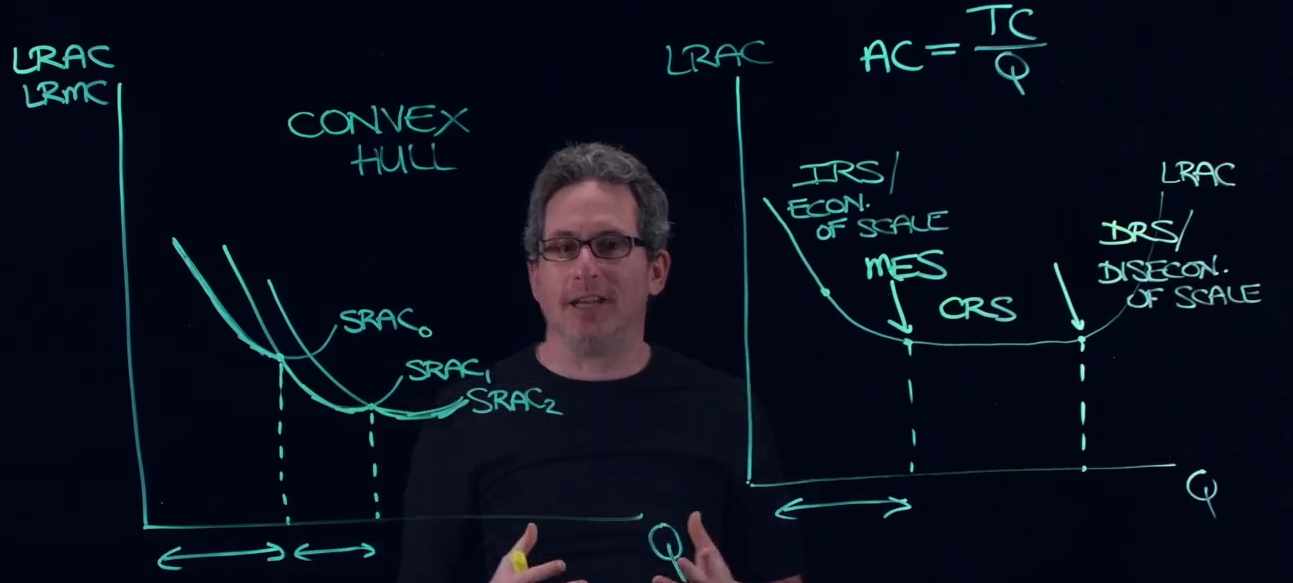
\includegraphics[width=0.5\textwidth]{./Chapter8/LongRunAverageCost.png}
\caption{Long Run Average Cost}
\end{figure}